\chapter[Theoretical Background and Methodology]{Theoretical Background and Methodology}
Molecular dynamics (MD) is a robust computational technique employed to explore the dynamic behaviour of atoms and molecules over time, offering microscopic insights into various physical and chemical phenomena. Its applications span diverse fields, including chemistry, physics, materials science, and biochemistry.

The origins of molecular dynamics can be traced back to the mid-20th century, with significant progress made in the following decades. Alder and Wainwright's pioneering work in the late 1950s laid the groundwork for numerically integrating classical equations of motion, enabling atomic-level simulations.\supercite{alder_studies_1959} Over time, computer hardware and algorithm advancements have propelled MD simulations to unprecedented accuracy and complexity.

The simulation entails solving Newton's equations of motion to predict the positions and velocities of atoms or molecules as they evolve. This computational approach yields valuable information on structural dynamics, thermodynamics, and kinetic properties of materials. The accuracy of MD simulations relies on the chosen force field, which mathematically models interactions between particles.

MD's significant contribution lies in unravelling the intricacies of biomolecular processes. Simulations of proteins, nucleic acids, and other macromolecules have proven invaluable for understanding protein folding, enzyme catalysis, and molecular recognition. These insights enhance our comprehension of molecular life and drive advancements in drug discovery and the design of targeted therapies.

Beyond biomolecules, MD plays a pivotal role in investigating the dynamics of solutions, enabling the study of liquids and gases in different environments. Its applications extend from understanding the properties of simple liquids to modelling complex solutions in chemical processes and environmental systems.

In summary, molecular dynamics offers a unique and powerful tool to investigate the dynamic nature of molecules and materials. Its applications across scientific domains drive advancements in our understanding of the natural world, facilitating the development of new technologies and solutions to complex problems.

In the context of this thesis, MD simulations were employed to investigate the dynamics of nucleobases, electrolyte solutions, and short ssDNA strands in the presence of a graphene surface. MD simulations involve solving Newton's equations of motion for numerous atoms at discrete time steps, generating a 3N-dimensional potential energy surface at each time slice, with the potential energy surface intricately tied to the atomic positions at each time step. The energy derivatives at each step are then utilized to propagate the coordinates and velocities to the subsequent step using one of the algorithms described below.

\section[Integration of Equations of Motion]{Integration of Equations of Motion}
\subsection[Integrators]{Integrators}
    \begin{itemize}
        \item \textbf{Verlet algorithm}\supercite{grubmuller_generalized_1991, gronbech-jensen_simple_2013}: The Verlet algorithm is a second-order integrator where the positions and velocities are propagated through time, starting from an initial set of coordinates and velocities. The Verlet algorithm is a numerically stable method. The algorithm is time reversible, meaning it is possible to run the integrator backwards to identify the dynamical trajectory's starting position due to the equations' lack of randomness. The basic algorithm does not require knowledge about the particle velocities to propagate the coordinates through time due to the algorithm's structure, which has a form described below.
        \begin{align*}
            x(1) &= x(0) + v(0)*\Delta t + \frac{1}{2}a(0)\Delta{t^2} \\
            x(t+1) &= 2x(t) - x(t-1) + a(t)\Delta{t^2}
        \end{align*}
        \item \textbf{Velocity-Verlet algorithm}\supercite{paterlini_constant_1998,marry_trotter_2007}: Velocity-verlet algorithm has explicit dependence on the velocities of the particles, and we use the velocities calculated at the midpoint of two consecutive timesteps in propagating the coordinates through time. The equations governing the Velocity-verlet algorithm have the form described below.
        \begin{align*}
            v(t + \frac{1}{2}\Delta{t}) &= v(t) + \frac{1}{2}a(t)\Delta{t} \\
            x(t+1) &= x(t) + v(t+ \frac{1}{2}\Delta{t})\Delta{t} \\
            a(t+1) &= F(t)/m \\
            v(t+1) &= v(t+\frac{1}{2}\Delta{t}) + \frac{1}{2}a(t+\Delta{t})\Delta{t}
        \end{align*}
        \item \textbf{Leapfrog algorithm}\supercite{toxvaerd_algorithms_1991,van_gunsteren_leap-frog_1988}: The Leapfrog algorithm is conceptually similar to the Velocity-verlet method in that positions and velocities leapfrog over each other in sequence. Similar to Verlet and Velocity-verlet algorithms, the leapfrog algorithm is also a second-order algorithm. 
    \end{itemize}

    \subsection{Constraints and Restraints}
    Traditionally, the bonds involving hydrogen atoms are constrained during an MD simulation, to allow for the ue of larger time steps in the integration of equations of motion. This is due to the fact that the time step of an MD simulation must be small enough to capture the fastest bond-stretching frequency, which would be for bonds involving hydrogen atoms.
    We use SETTLE\supercite{miyamoto_settle_1992} and SHAKE\supercite{ryckaert_numerical_1977} algorithms to constraint the necessary bonds in the MD simulations.

    When employing constraints, they are generally employed using lagrange multipliers, where the are $n$ holomonic constraints denoted as $\left\{ \sigma_1,\sigma_2,\cdots  \right\}$, we can express the lagrange multipliers as:
    \begin{align*}
        \sigma_k = \left\| r_i(t) - r_j(t)\right\|^2 - d_k^2
    \end{align*} 

    where $\sigma_k$ is the $k^{th}$ holonomic constraint, and $r_i$ and $r_j$ are the unconstrained positions of $i^{th}$ and $j^{th}$ atom involved in the $k^{th}$ holonomic constraint, and $d_{k}$ is the constrained bond length.

    In contrast, Restraints are generally applied to restrain one (or more) atoms in space. This is generally employed by attaching a spring on the restrained atom (atoms) with a user defined spring constant, such that the motion of the restrained atoms is arrested during the MD simulations. This is particulary useful when investigating surfaces, where you need to account for the surface vibrations, but also need to arrest the sliding motion of the surface.

    \subsection{Thermostats and Barostats}
    Thermostats and Barostats are typically employed to investigate a system in a particular ensemble (isobaric-isothermal or isochoric-isothermal), and a selection of thermostats and barostats which can be used for the same are described below: 

    \begin{itemize}
        \item \textbf{Velocity rescaling Thermostat}\supercite{woodcock_isothermal_1971}: This is the simplest form of themostat, where the atomic velocities at each step are rescaled by a factor $\lambda$ at a calculated temperature of $T(t)$, such that the rescaled velocities are at the desired temperature $T_0$.
        \begin{align*}
            \lambda = \sqrt{\frac{T(t)}{T_0}}
        \end{align*}

        \item \textbf{Berendsen Thermostat}\supercite{berendsen_molecular_1984}: In Berendsen Thermostat, the system is weakly coupled to an external heat bath, with an associated coupling constant $\tau$, such that the velocities at each step are rescaled by a parameter $\lambda$. Here, the temperatures are alloed to fluctuate, but the temperature $T(t)$ is dampened towards the target temperature $T_0$.
        \begin{align*}
            \lambda = \sqrt{\left[1 + \frac{dt}{\tau}\left(\frac{T_0}{T(t)}-1\right)\right]}
        \end{align*}

        \item \textbf{Andersen Thermostat}\supercite{andersen_molecular_1980}: In Andersen Thermostat, a predertmined number of atoms undergo collision with a stochastic bath particles, and are then assigned new velocities based on the Maxwell-Boltzmann distribution such that the canonical ensemble is correctly sampled. The time interval between two successive collisions is dependent on the collision frequency ($\nu$) and follows the Poisson distribution.

        \item \textbf{Langevin Thermostat}\supercite{schneider_molecular-dynamics_1978}: Langevin dynamics controls the system's temperature by introducing a Gaussian random error term, which readjusts the particles' velocities via collisions with virtual particles modelled via Gaussian random errors. However, the presence of this error term means that Langevin dynamics is not time-reversible, unlike other algorithms.
        \begin{align*}
            \ddot{r_i} = \frac{F_i - m_i\gamma v_i + F^{rand}_i}{m_i}
        \end{align*}
        Here, $\ddot{r}$ denotes the accelaration on the particle $i$, $\gamma$ denotes the friction coefficient, and $F^{rand}_i$ in a Gaussian random error term with a mean of zero and non-zero $\sigma$ calculated as:
        \begin{align*}
            \sigma_i = \sqrt{\frac{2m_i\gamma k_B T}{dt}}
        \end{align*}

        \item \textbf{Nos\'{e}-Hoover Thermostat}\supercite{nose_molecular_1984,hoover_canonical_1985}: In Nos\'{e}-Hoover Thermostat, the system is extended via the introduction of a virtual particle $\bar{s}$ with a mass $Q > 0$ and a velocity of $\dot{\bar{s}}$, with the magnitude of $Q$ determining the coupling between the heath bath and the system, and in turn determining the temperature fluctuations. The Hamiltonian for the extended system can then be written as:
        \begin{align*}
            \mathcal{H} = \frac{P_i^2}{2m_i} + U(r) + \frac{p_s^2}{2Q} + N_{free}k_BTln(s) 
        \end{align*}
        where $N_{free}$ is the available number of degrees of freedom.
    \end{itemize}

    Having discussed the available Thermostats, we now discuss the available Barostats.
    \begin{itemize}
        \item \textbf{Berendsen Barostat}\supercite{berendsen_molecular_1984}: In Berendsen Barostat, the coordinates and the cell vectors are rescaled at each time step, with the pressure $P(t)$ relaxing to a target pressure $P_0$ following the first order kinetic equation:
        \begin{align*}
            \frac{dP(t)}{dt} = \frac{P-P_0}{\tau_p}
        \end{align*}
        where $P(t)$ is the instantaneous pressure, $P_0$ is the target pressure and $\tau_p$ is the barostat relaxation time. 

        Here, the scaling matrix for the cell vectors is determined from the following equation:
        \begin{align*}
            \mu = 1 - \frac{dt\beta}{\tau_p}\left(P_0 - P(t)\right)
        \end{align*}
        where $\beta$ is the isothermal compressiblity of the system, and is usually set to a value of $4.6x10^{-10}$ Pa\textsuperscript{-1} which is the isothermal compressiblity of liquid water at 300 K and 1 atm pressure. The matrix $\mu$ will be diagonal with the elements $\mu_{xx} = \mu_{yy} = \mu_{zz}$ if the scaling is isotropic.

        \item \textbf{Nos\'{e}-Hoover Langevin Barostat}\supercite{feller_constant_1995,martyna_constant_1994}: In Nos\'{e}-Hoover Langevin Barostat, the pressure control in implemented via the use of Langevin dynamics to control the pressure fluctuations. In this algorithm, the pressure fluctuations are introduced by using langevin equation where V is also a dynamical variable, of the form:
        \begin{align*}
            \dot{r_i} &= \frac{p_i}{m_i} + \frac{1\dot{V}}{3V}r_i \\
            p_i &= f_i - \frac{\dot{V}}{3V}p \\
            \ddot{V} &= \frac{1}{Q}\left[P(t)-P_0\right]-\gamma\dot{V} + R(t)
        \end{align*}

        where $Q$ is the mass of the virtual particle, $P(t)$ is the instantaneous pressure and $P_0$ is the target pressure. Here $\gamma$ is the collision frequency, and $R(t)$ is the Gaussian random noise.
    \end{itemize}

    \subsection{Short-range and Long-range Interactions}
    From a computational standpoint, the evaluation of the non-bonded interactions are the most expensive, with a naive algorithm scaling as $N^2$ where $N$ is the number of particles in the system. One of the easiest methods to reduce the associated computational complexity is to use a cut-off scheme, where the interactions between two particles are smoothly varied to zero, depending on some distance based criterion. We present a representative image depicting the distance based cut-off scheme in Figure 2.1. 
    \begin{figure}[!h]
        \centering
        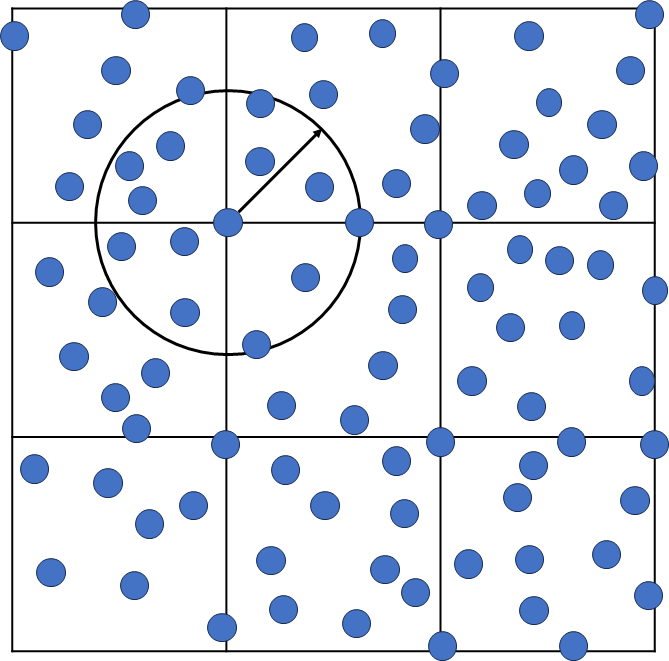
\includegraphics[width=0.5\textwidth]{Methods/Figures/cutoff.png}
        \caption[Representative Image depicting the use of a distance based cut-off scheme for the evaluation of non-bonded interactions]{Representative Image depicting the use of a distance based cut-off scheme for the evaluation of non-bonded interactions. Blue spheres indicate Helium atoms, and the black circle indicates the cut-off sphere for the evaluation of non-bonded interactions.}
    \end{figure}
    
    Here, the distance-based cut-off would be a sufficiently reasonable approximation in the evaluation of short-range VdW interactions, however for long-range interactions such as electrostatics, this approximation would introduce large errors in the evaluated energies due to the slow onvergence. One method to mitigate this problem is the use of Ewald summation, wherein the electrostatic interactions is decomposed into two terms: one term in real-space that converges very quickly, and a long-range term summing over the periodic images. However, Ewald summation might face convergence issues, if either the unit cell is ill-defined, or the unit-cell is not charge neutral. 
    
    In Particle Mesh Ewald (PME) method, the electrostatic interaction is again decomposed into two terms: a short-range term evaluated in real-space, and a long-range term evaluated in fourier space. In PME, the long-range term is evaluated on a discrete mesh of charges, and is evalued using FFT algorithms. As in the case of Ewald summation, PME also requires the simulation to be periodic in x-,y- and z-directions, and have a smoothly varying density.
    
    \subsection{Periodic Boundary Conditions}
    It is computationally impractical to perform MD simulations on systems of experimentally relevant dimensions. Periodic boundary conditions (PBC) allow us to use a simulation box of computationally trackable dimensions and mitigate finite box effects like self-interactions. Under periodic boundary conditions, any particle leaving the box during the simulation is replaced by its image from one of the twenty-six periodic images generated around the original simulation box. We present a representative image depicting the PBC conditions in a 2D plane in Figure 2.2.

    \begin{figure}[!h]
        \centering
        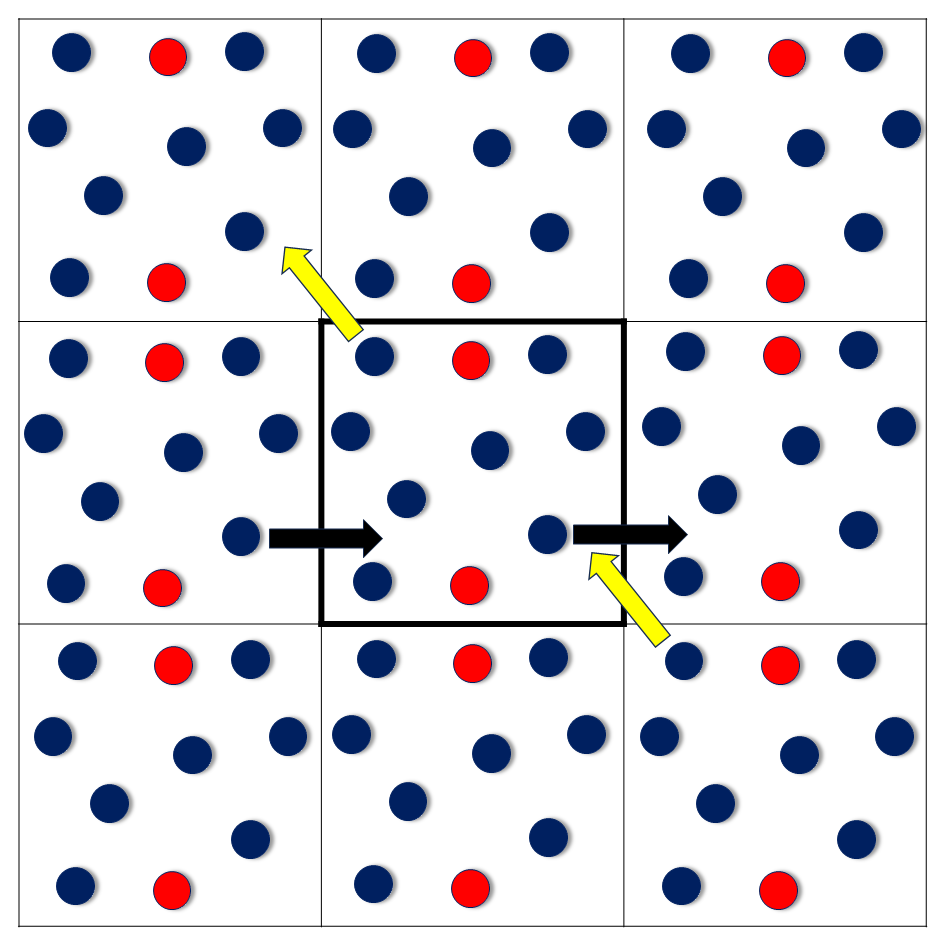
\includegraphics[width=0.5\textwidth]{Methods/Figures/pbc.png}
        \caption[Representative image depicting the application of PBC in a 2D plane]{Representative image depicting the application of PBC in a 2D plane. The central simulation box is indicated by the use of solid lines. The trajectory for two particles at the edges of the simulation box, and its periodic images are also indicated.}
    \end{figure}

    % Consider the case of a 3D system with system dimensions of Lx, Ly and Lz and angles of 90. A naive implementation for the periodic boundary conditions in Fortran, in this case, would be as follows:
    % \begin{align*}
    %     r &= r - r_{old}        \\           
    %     r &= r - \text{ANINT}( \frac{r}{box}) * box \\
    % % r &= r + r_{old}               \\    
    % \end{align*}

    % Here $r$ and $r_{old}$ are the coordinates of the particle at time $t+1$ and $t$, and ANINT is a Fortran routine that rounds a floating point number to the nearest integer.

    \section{Force fields}
    The fundamental idea behind FFs is to decompose the interactions between collections of atoms into a set of analytic functions fitted to reproduce QM results and (or) experimental observables. We can decompose the interactions between sets of atoms into the following sections:
    \begin{itemize}
        \item We model all atoms as hard spheres, and Hook's law models the bonds between atoms, where the bond is approximated with a spring of a specified spring constant, empirically determined. 
        \item We use Hook's law to model angles between three bonded atoms, where the spring constant determines the flexibility of the angle and is also empirically determined. 
        \item We use a periodic potential to model the dihedral between four bonded atoms since the dihedral angle is between [0,180]. 
        \item The standard Lennard-Jones equation evaluates non-bonded interactions between all pairs of non-bonded atoms.
    \end{itemize}
    One central assumption is that the parameters are molecule-agnostic, i.e. the parameters developed for one set of atoms can be transferred with minimal reparameterization towards another molecule, provided the chemical environment of the atom is equivalent. In other words, the parameters used to describe a carbon atom in benzene must be transferrable to describe the carbon atom in naphthalene in a similar chemical environment, with the parameters requiring minimal modifications.
    
    We have employed Chemistry at HARvard Molecular Mechanics (CHARMM) FF for the simulations reported in this thesis. The functional form of the classical non-polarizable additive FF is as follows:
    \begin{multline*}
        V(r^N) = \sum_{bonds}^{}k_i(x_i-x_i^{min})^2 + \sum_{angles}^{}k_j(\theta_j-\theta_j^{min})^2 + \sum_{dihedrals}^{}k_{\phi}(1 + cos(n\phi-\delta)) + \\ \sum_{impropers}^{} k_{\omega}(\omega - \omega_{min})^2 + \sum_{UreyBradley}^{}(S-S_{min})^2 + \\ \sum_{electrostatic}^{}\frac{1}{\epsilon}*\frac{q_i * q_j}{r_{ij}} +  \sum_{VdW}^{}\epsilon_{ij}(\frac{\sigma_{ij}^{12}}{r_{ij}^{12}}-\frac{\sigma_{ij}^{6}}{r_{ij}^6})
    \end{multline*}
    
    where $k_i$, $k_j$ etc are the spring constants for the bonds and angles respectively. Values indicated as $x_{i}^{min}$, $\theta_{i}^{min}$ correspond to the equilibrium bond length and angle. As observed from the equation, the dihedral energy is expressed as the linear combination of a periodic cosine function, where $k_{\phi}$ is the force constant, $\phi$ is the dihedral angle, $\delta$ is the phase shift, and $n$ is the multiplicity of the dihedral. Improper dihedrals are important in maintaining the planarity of a structure, where $k_{\omega}$ is the spring constant and $\omega$ characterizes the out-of-plane bend of the plane. Urey-Bradley interactions account for the 1-3 interactions between the $i^{th}$ and $k^{th}$ atoms in an angle formed by i, j and k atoms, and has important applications in maintaining the geometry of H-O-H angle in water. VdW interactions between two non-bonded atoms i and j, separated by a distance $R_{ij}$ is evaluated using a pairwise Lennard-Jones potential dependent on the specific ``well-depth'' $(\epsilon)$ and equilibrium distance $\sigma$ for the interating particles. The energy terms are evaluated using the standard Lorentz-Berthelot mixing rules:
    \begin{align*}
        \sigma_{ij} &=   \frac{\sigma_i + \sigma_j}{2} \\
        \epsilon_{ij} &= \sqrt{\epsilon_i*\epsilon_j}
    \end{align*}

    Electrostatic energy is computed using Coulumb potential, with $q_i$ and $q_j$ being the partial charges on the particles, and $r_{ij}$ being the distance between the particles.

    \subsection[Classical Drude FF]{Classical Drude FF}
    We have also used classical Drude polarizable FF to investigate the influence of polarizability on the dynamics of the systems. Here, we note that classical non-polarizable FFs like CHARMM have their basis in fixed-point charges, which means that they are not particularly suited for studying systems where significant shifts in the local environment for the molecules are expected, like in the case of biological systems. In such cases, polarizable FFs like classical Drude polarizable FF offers a pathway towards the inclusion of the contributions from the local environment towards the dynamics of the systems.

    In the case of classical Drude polarizable FF, the polarizability of the heavy atoms (excluding hydrogen) is modelled via Drude particles attached to the heavy atoms via a harmonic spring. The Drude particles have a negative charge associated with them. In contrast, the atomic cores have a positive charge, such that the total charge of the atom and associated Drude particle equals the partial charge of the atom. A representative structure depicting the arrangement of atomic cores and associated drude particles are presented in Figure 2.3. 
    \begin{figure}
        \centering
        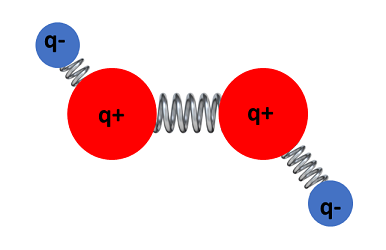
\includegraphics[width=0.75\textwidth]{Methods/Figures/drude.png}
        \caption[Schematic Representation of Drude particles for a C-C bond]{Schematic Representation of Drude particles for a C-C bond. Carbon atoms are represented as red speheres, and Drude particles are represented as blue spheres. The partial positive and negative charges of the heavy atoms and the Drude particles are also indicated. Bonds between heavy atoms are represented as larger springs, and bonds between Drude particles and heavy atoms are represented using smaller springs.}
    \end{figure}

    Here, the Drude particles represent the electronic degrees of freedom for the heavy atom, with the vibration of the Drude particle allowing the electronic interactions of the heavy atom to respond to fluctuations in the local environment, via dipole-dipole and induced-dipole effects. In classical Drude FF, the charges on the Drude particles ($q_D$) and the induced dipole moment ($\mu$) in an external electric field \textit{E} is defined as:
     \begin{align*}
        \mu &= \frac{{q_D}^2 E}{k_d}\\
        d &= \frac{q_D E}{k_d}
     \end{align*}

     We evalue the atomic polarizability ($\alpha$) as:
     \begin{equation*}
        \alpha  =   \frac{{q_D}^2}{k_d}
     \end{equation*}

    Here, the value of $k_D$ corresponds to the harmonic spring constant for the bond connecting the Drude particle to the heavy atom, and has a value of 1000 kcal mol\textsuperscript{-1} for all Drude particle-heavy atom pairs, while a value of 500 kcal mol\textsuperscript{-1}, corresponding to $\frac{k_D}{2}$ is used in CHARMM and NAMD.

    The bonded and non-bonded terms in classical Drude FF is treated exactly the same as in non-polarizable additive FF, with the functional form of the interactions remaining the same in both the FF. The electrostatic interactions are calculated using the following functional form, to include the effects of the electrostatic interactiosn between the unscreened charges, and the Drude particles on $i^{th}$ and $j^{th}$ atom. 
    \begin{align*}
        U_{elec} = \sum_{i}^{}\sum_{j>i}^{}\left[\frac{q_i * q_j}{|r_i - r_j|} + \frac{q_i * q_{D_j}}{|r_i - r_j - d_j|} + \frac{q_j * q_{D_i}}{|r_j - r_i - d_i|} + \frac{q_{D_i} * q_{D_j}}{|r_i - d_i - r_j - d_j|}\right]
    \end{align*}

    Here, $q_i$ and $q_j$ correspond to the unscreened charges on the heavy atoms, while $q_{D_i}$ and $q_{D_j}$ correspond to the charges on the corresponding Drude particles. $r_i$, $r_j$, $d_i$ and $d_j$ are the locations of the $i^{th}$ and $j^{th}$ heavy atoms and the associated Drude particles. The electrostatic term includes the induced-dipole interaction between the two interacting atoms, and 1-2 and 1-3 atom interactions are scaled according to the Thole scaling function, which is described below:
    \begin{align*}
        S_{ij}(r_{ij}) = 1 - \left| 1 + \frac{(a_i * a_j)*r_{ij}}{2(\alpha_i*\alpha_j)^{\frac{1}{6}}}*\exp{\left[\frac{(a_i * a_j)*r_{ij}}{(\alpha_i * \alpha_j)^{\frac{1}{6}}}\right]} \right|
    \end{align*} 

    Here, $r_{ij}$ is the distance between the $i^{th}$ and $j^{th}$ atom, and $a_i$ and $a_j$ are the corresponding thole screeing parameters.

    Classical Drude FF has been employed to investigate the dynamics of a wide variety of systems; including carbohydrates\supercite{pandey_drude_2019,kognole_extension_2022}, proteins and nucleic acids; and contains the parameters to describe a large subset of the chemical space including, but not limited to; biomolecules\supercite{baker_development_2011,savelyev_all-atom_2014}, ions\supercite{lin_polarizable_2018}, water\supercite{lamoureux_polarizable_2006}, heteroatom (O-, N- and S-) conatining molecules\supercite{lopes_polarizable_2009,zhu_polarizable_2010,he_polarizable_2013}, linear and branched hydrocarbons\supercite{vorobyov_polarizable_2005} and aromatic compounds\supercite{lopes_polarizable_2007}.

    We also note that the availabity of classical Drude FF in MD simulation packages like CHARMM\supercite{brooks_charmm_1983,brooks_charmm_2009}, NAMD\supercite{phillips_scalable_2005,phillips_scalable_2020} and OpenMM\supercite{eastman_openmm_2010,eastman_openmm_2017} enables the study of large systems of experimental and biological relevance using MD simulations, without the need to use expensive QM/MM or ab-initio dynamics methods.

The quality of a molecular dynamics simulation is highly dependent on multiple factors, in which three factors listed below are of significant importance:
\begin{itemize}
    \item Initial positions of the atoms in the starting structure. If the intial confirmations introduce some biases in the system, it would affect the simulations outcomes, such that all possible states might not get adequately sampled during the simulation.
    \item Parameters used to describe the interactions between the particles (atoms) during the MD simulation, which are used to compute the potential energy surface. If the parameters used are unable to describe certain interactions, the predictions might not be reflective of the experimental observations.
    \item Integrator used to propagate the structure from time step of $t$ to time step of $t+1$. Some integrators might be numerically unstable over large lengths of time, and the errors at each step might get accumulated in the trajectory.
\end{itemize}

\section{Adaptive Biasing Force Simulations}
We employed Adaptive Biasing Force (ABF) simulations to investigate the binding energies of small molecules with the graphene surface in additive and classical Drude FF simulations. Here, we briefly describe the ABF method and then discuss the specific use case given in this thesis.

ABF, at its core, is an importance sampling method\supercite{comer_adaptive_2015}. However, the importance is adaptive, such that the code can automatically adjust the average force to escape kinetic energy traps in the free-energy surface. In ABF, the free energy along a transition coordinate (called a collective variable) is the negative gradient of the potential arising from the average force acting along that transition coordinate ($\xi$). The force acting on the system can be decomposed into two terms: one corresponding to the average force acting on it and the other term accounting for the random force amounting to the fluctuations in all other degrees of freedom for the system. Here, the random force is thought of as a diffusive force, such that the system under investigation evolves diffusively along the path of the potential of the mean force. The adaptive nature of the ABF method lies in the fact that the method requires no information about the free energy surface apriori, and the derivative of the free energy (and the path of diffusion) is estimated on the fly during the simulation. The method accomplishes this by estimating the running average of the instantaneous force acting on the system and applying an equal and opposite external bias, such that the sum of both forces is zero. Since the average applied external bias would converge to zero over time, and the running average of the instantaneous force on the system converges to the average value at equilibrium, the system now has a flat potential energy landscape, where the remaining barriers would be overcome via thermal fluctuations.

Mathematically, the ABF method works by modifying the potential V to resemble a flat energy landscape along the transition coordinate ($\xi$) of our choice, such that $V(x)$ becomes $V(x) - A_t[\xi(x)]$. We then update $A_t$ such that it converges to the free energy $A$, with the difference of an additive constant, as defined by:
\begin{align*}
    \exp(\beta A(z)) = \int_{}^{}\exp\left[-\beta V(x)\right]\delta_{\xi(x)-z}(dx)
\end{align*}
where $\delta_{\xi(x)-z}(dx)dz = dx$.

We now look into the update rule for $A_t$ such that the condition $\lim_{t\to\infty} A_t = A$ holds true. We have the formula
\begin{align*}
    A'(z) &= -\frac{\int F_{\xi}(x)\exp\left[-\beta V(x)\right]\delta_{\xi(x)-z}(dx)}{\int\exp\left[-\beta (x)\right]\delta_{\xi(x)-z}(dx)} \\
    F_\xi &= -\frac{\nabla V.\nabla\xi}{\left| \nabla\xi \right|^2} + \beta^{-1} div\left(\frac{\nabla\xi}{\left| \nabla\xi \right|^2}\right)
\end{align*}

We now note that $A'(z)$ denotes the conditional average of $F_\xi$, and the equation for $A'(z)$ remains true even when the potential is changed to $V(x) - A_t\circ\xi$ for any function $A_t$. Thus, we note that a biasing potential $A_t$ that depends only on the $\xi$, will leave avergaes conditioned by $\xi$ the same. Tthe logic behind ABF method can be summarized as follows:
\begin{align*}
    dx_t &= M^{-1} p_t dt \\
    dp_t &= -\nabla(V - A_t\circ\xi)(x_t)dt - \gamma M^{-1}p_tdt + \sqrt{2\gamma k_BT}dW_t \\
    A'_t(z) &= E\left[F_\xi(x_t)|\xi(x_t)=z\right]
\end{align*}
where $x_t$ and $p_t$ are the position and momentum of the system at time $t$, $M$ is the mass tensor, $k_B$ is the boltzmann constant, and $W_t$ is the Gaussian random process.

It is recommended that the collective variable $\xi$ be split into multiple windows, so that convergence towards the average value is accelerated.

In this thesis, we employed ABF simulations to investigate the potential of mean force for the interactions between the nucleobases and the graphene surface in Chapter3, between monovalent and divalent cations and Cl\textsuperscript{-1} ion with the graphene surface in Chapter5, and between nucleosides and modified nucleotides and graphene surface in Chapter6. In all these calculations, the collective variable $(\xi)$ was chosen to be the z-projected distance between the graphene surface and the center of mass of the small molecule (nucleobases, nucleosides or modified nucleotides) or ions.

\section{Software and Hardware Used}
This thesis employed the Nanoscale Molecular Dynamics (NAMD) simulation package to perform all classical MD simulations. The initial QM calculations reported in the first chapter used Gaussian 09 and Orca. Home-developed Python codes were also utilized to conduct all the analyses reported herein. All MD trajectories and PDB structures were visualized using the Visual Molecular Dynamics (VMD) and GaussView packages. This thesis required extensive computational resources provided by the High-Performance Computing Facility, IIT Gandhinagar, and Param Ananta Supercomputing Facility at IIT Gandhinagar. 